\documentclass[conference]{IEEEtran}
%\usepackage{llncsdoc}
\usepackage{graphicx}
\usepackage{amssymb}
\usepackage{algorithm}
\usepackage[noend]{distribalgo}

\newcommand{\ex}{$\mathcal{E}$}
\newcommand{\pp}{$\mathcal{P}$}
\newcommand{\ppm}{\mathcal{P}}
\newcommand{\cc}{$\mathcal{C}$}
\newcommand{\ccm}{\mathcal{C}}
\newcommand{\vv}{$\mathcal{V}$}
\newcommand{\vvm}{\mathcal{V}}
\newcommand{\vvt}{$\mathcal{V}$}
\newcommand{\rr}{$\mathcal{R}$}
\newcommand{\rrm}{\mathcal{R}}
\newcommand{\sst}{$\mathcal{S}$}
\newcommand{\ssm}{\mathcal{S}}
%
\newcommand{\ssmr}{\mbox{S-SMR}}
\newcommand{\dssmr}{\mbox{DS-SMR}}
%
\newcommand{\rmcast}{reliable-multicast}
\newcommand{\rmdel}{reliable-deliver}
\newcommand{\amcast}{atomic-multicast}
\newcommand{\amdel}{atomic-deliver}
\begin{document}

\title{Dynamic Scalable State Machine Replication}

\author{\IEEEauthorblockN{Long Hoang Le}
\IEEEauthorblockA{University of Lugano\\Switzerland}
\and
\IEEEauthorblockN{Carlos Eduardo Bezerra}
\IEEEauthorblockA{University of Lugano\\Switzerland}
\and
\IEEEauthorblockN{Fernando Pedone}
\IEEEauthorblockA{University of Lugano\\Switzerland}}

\maketitle
%
\begin{abstract}
%Borrow from SSMR paper

%State machine replication (SMR) is a well-known technique to provide high availability and strong consistency (i.e., linearizability) to online services.
%In SMR, client commands are executed in the same order on all server replicas: after executing each client command, every replica will reach the same state. 
%%
%One problem is that the original SMR model lacks scalability, as every replica executes all commands.
%Because of that, adding replicas does not increase the maximum system throughput.
%%
%Scalable SMR (\ssmr) addresses this problem by partitioning the service state, allowing client commands to be executed only by some replicas, while still ensuring linearizability.
%By doing this, \ssmr\ scales linearly with the number of partitions for workloads where each command accesses a single partition.
%%
%However, \ssmr\ may quickly become saturated when executing multi-partition commands,
%as they require communication between partitions.
%Dynamic S-SMR (\dssmr) solves this problem by repartitioning the state dynamically, based on the workload.
%When a command needs variables from different partitions, those variables are first moved to the same partition.
%Then, the command is executed as a single-partition command.
%As a result, variables that are usually accessed together will tend to stay in the same partition, significantly improving scalability.
%We evaluate the performance of \dssmr\ with a scalable social network application.

State machine replication (SMR) is a well-known technique that guarantees strong consistency (i.e., linearizability) to online services.
In SMR, client commands are executed in the same order on all server replicas: after executing each command, every replica reaches the same state.
However, SMR lacks scalability: every replica executes all commands, so adding servers does not increase the maximum throughput.
Scalable SMR (\ssmr) addresses this problem by partitioning the service state, allowing commands to execute only in some replicas, providing scalability while still ensuring linearizability.
One problem is that ssmr quickly saturates when executing multi-partition commands,
as partitions must communicate.
\dssmrshort\ (\dssmr) solves this issue by repartitioning the state dynamically, based on the workload.
Variables that are usually accessed together are moved to the same partition, which significantly improves scalability.
We evaluate the performance of \dssmr\ with a scalable social network application.

\end{abstract}
%!TEX root =  main.tex
\section{Introduction}

State machine replication (SMR) is a well-established technique to develop highly available services (e.g., \cite{Shvachko:2003,Ghemawat:2003,Burrows:2006,MacCormick:2004}).
In essence, the idea is that replicas deterministically execute the same sequence of client commands in the same order and in doing so traverse the same sequence of states and produce the same results.
State machine replication provides configurable fault tolerance in the sense that the system can be set to tolerate any number of faulty replicas.
%Increasing the number of replicas, however, will not scale performance since each replica must execute every command.
Unfortunately, increasing the number of replicas will not scale performance since each replica must execute every command.

%For many online services, caping performance is a serious drawback.
Conceptually, scalable performance can be achieved with state partitioning (e.g., \cite{facebookTAO, sciascia2012sdur, Aguilera:2007}).
Ideally, if the service state can be divided such that commands access one partition only and are equally distributed among partitions, then system throughput (i.e., the number of commands that can be executed per time unit) will increase linearly with the number of partitions.
Although promising, exploiting partitioning in SMR is challenging.
First, most applications cannot be partitioned in such a way that commands always fall within a single partition.
Therefore, a partitioning scheme must cope with multi-partition commands.
Second, determining an efficient partitioning of the state is computationally expensive and requires an accurate characterization of the workload.

There are two general solutions to handle multi-partition commands.
One solution is to weaken the guarantees of commands that involve multiple partitions (e.g., \cite{facebookTAO}).
In the context of SMR, this would mean that single-partition commands are strongly consistent (i.e., linearizable) but multi-partition commands are not.
Another solution is to provide strong consistency guarantees for both single- and multi-partition commands, at the cost of a more complex execution path for commands that involve multiple partitions.
\ssmrlong\ (\ssmr)~\cite{bezerra2014ssmr} is a solution in this category.
\ssmr\ partitions the service state and replicates each partition.
It relies on an atomic multicast primitive to consistently order commands within and across partitions. 
Single-partition commands are multicast to their concerned partition and executed just like in classical SMR.
Multi-partition commands are multicast to all involved partitions; to prevent command interleaves that violate strong consistency, \ssmr\ implements execution atomicity.
With execution atomicity, partitions coordinate during the execution of multi-partition commands.
Unsurprisingly, multi-partition commands are more expensive than single-partition commands, and thus, the performance of \ssmr\ is particularly sensitive to the way the service state is partitioned.

Determining a partitioning of the state that avoids load imbalances and favors single-partition commands normally requires a good understanding about the workload. 
Even if enough information is available, finding a good partitioning is a complex optimization problem~\cite{curino2010sch,taft2014est}.
Moreover, many online applications experience variations in demand. 
These happen for a number of reasons. 
In social networks, some users may experience a surge increase in their number of followers (e.g., new ``celebrities");
workload demand may shift along the hours of the day and the days of the week; and unexpected (e.g., a video that goes viral) or planned events (e.g., a new company starts trading in the stock exchange) may lead to exceptional periods when requests increase significantly higher than in normal periods.
\ssmr\ assumes a static workload partitioning.
Any state reorganization requires system shutdown and manual intervention.

Given these issues, it is crucial that highly available partitioned systems be able to dynamically adapt to the workload.
In this paper, we present \dssmrlong\ (\dssmr), a technique that allows a partitioned SMR system to reconfigure its data placement on-the-fly.
\dssmr\ achieves dynamic data reconfiguration without sacrificing scalability or violating the properties of classical SMR.
These requirements introduce significant challenges.
Since state variables may change location, clients must find the current location of variables.
The scalability requirement rules out the use of a centralized oracle that clients can consult to find out the partitions a command must be multicast to.
Even if clients can determine the current location of the variables needed to execute a command, by the time the command is delivered at the involved partitions one or more variables may have changed their location.
Although the client can retry the command with the new locations, how to guarantee that the command will succeed in the second attempt?
In classical SMR, every command invoked by a non-faulty client always succeeds.
\dssmr\ should provide similar guarantees.

\dssmr\ was designed to exploit workload locality.
Our scheme benefits from simple manifestations of locality, such as commands that repeatedly access the same state variables, and more complex manifestations, such as structural locality in social network applications, where users with common interests have a higher probability of being interconnected in the social graph.
Focusing on locality allows us to adopt a simple but effective approach to state reconfiguration: whenever a command requires data from multiple partitions, the variables involved are moved to a single partition and the command is executed against this partition.
To reduce the chances of skewed load among partitions, the destination partition is chosen randomly.
Although \dssmr\ could use more sophisticated forms of partitioning, formulated as an optimization problem (e.g., \cite{curino2010sch,taft2014est}), our technique has the advantage that it does not need any prior information about the workload and is not computationally expensive.

To track object locations without compromising scalability, in addition to a centralized oracle that contains accurate information about the location of state variables, each client caches previous consults to the oracle.
As a result, the oracle is only contacted the first time a client accesses a variable or after a variable changes its partition.
Under the assumption of locality, we expect that most queries to the oracle will be accurately resolved by the client's cache.
To ensure that commands always succeed, despite concurrent relocations, after attempting to execute a command a few times unsuccessfully, \dssmr\ retries the command using \ssmr{}'s execution atomicity and involving all partitions. 
Doing so increases the cost to execute the command but guarantees that relocations will not interfere with the execution of the command.

We have fully implemented \dssmr\ as the \libname{} Java library, and we performed a number of experiments using \appname{}, a social network application built with \libname{}, with workloads exhibiting weak and strong locality.
We devised a mixed workload that estimates a real distribution of commands issued in a social network application.
Under such a workload, and with strong locality of access, \dssmr\ reached 74~kcps (thousands of commands per second), against less than 33~kcps achieved by \ssmr{}, improving by a factor of over 2.2.
With a weak-locality workload, \dssmr\ reached XX~kcps, against YY~kcps of \ssmr{}.

The paper makes the following contributions:
(1) It introduces \dssmr\ and discusses some performance optimizations, including the caching technique. 
(2) It details \libname{}, a Java library to simplify the design of services based on \dssmr{}.
(3) It describes \appname{} to demonstrate how \libname{} can be used to implement a scalable social network service.
(4) It presents a detailed experimental evaluation of \appname{}, deploying it with \ssmr\ and \dssmr{} in order to compare the performance of the two replication techniques.

The rest of the paper is structured as follows.
Section~\ref{sec:sysmodel} describes our system model.
Section~\ref{sec:background} reviews SMR and \ssmrshort{}.
Section~\ref{sec:dssmr} introduces \dssmr{}; we explain the technique in detail and argue about its correctness.
Section~\ref{sec:implementation} details the implementation of \libname\ and \appname{}.
Section~\ref{sec:experiments} reports on the results of our experiments with \dssmr{}.
Section~\ref{sec:rw} surveys related work and
Section~\ref{sec:conclusion} concludes the paper.






\clearpage
\section{System model and definitions}
\label{sec:sysmodel}

We consider a distributed system consisting of an unbounded set of client processes $\ccm = \{c_1, c_2, ...\}$ and a bounded set of server processes (replicas) $\ssm = \{s_1, ..., s_n\}$. 
Set $\ssm$ is divided into disjoint groups of servers $\ssm_0, ..., \ssm_k$.
Processes are either \emph{correct}, if they never fail, or \emph{faulty}, otherwise. 
In either case, processes do not experience arbitrary behavior (i.e., no Byzantine failures).

Processes communicate by message passing, using either one-to-one or one-to-many communication.
The system is asynchronous: there is no bound on message delay or on relative process speed.
One-to-one communication uses primitives $send(p,m)$ and $receive(m)$, where $m$ is a message and $p$ is the process $m$ is addressed to. 
If sender and receiver are correct, then every message sent is eventually received. 
%
One-to-many communication relies on reliable multicast and atomic multicast,\footnote{Solving atomic multicast requires additional assumptions~\cite{CT96,FLP85}. In the following, we simply assume the existence of an atomic multicast oracle.}
defined in sections~\ref{sec:rmcast} and \ref{sec:amcast}, respectively.
%Atomic broadcast is a special case of atomic multicast in which there is a single group with all servers.

Our consistency criterion is linearizability.
A system is \emph{linearizable} if there is a way to reorder the client commands in a sequence that (i)~respects the semantics of the commands, as defined in their sequential specifications, and (ii)~respects the real-time precedence of commands~\cite{Attiya04}.

\subsection{Reliable multicast}
\label{sec:rmcast}

To reliably multicast a message $m$ to a set of groups $\gamma$, processes use primitive \rmcast$(\gamma, m)$.
Message $m$ is delivered at the destinations with \rmdel$(m)$.
Reliable multicast has the following properties:

\begin{itemize}

    \item[--] If a correct process \rmcast{}s $m$, then every correct process in $\gamma$ \rmdel{}s $m$ \emph{(validity)}.
    
    \item[--] If a correct process \rmdel{}s $m$, then every correct process in $\gamma$ \rmdel{}s $m$ \emph{(agreement)}.
    
    \item[--] For any message $m$, every process $p$ in $\gamma$ \rmdel{}s $m$ at most once, and only if some process has \rmcast{} $m$  to $\gamma$ previously \emph{(integrity)}.
    
\end{itemize}

\subsection{Atomic multicast}
\label{sec:amcast}

To atomically multicast a message $m$ to a set of groups $\gamma$, processes use primitive \amcast$(\gamma, m)$.
Message $m$ is delivered at the destinations with \amdel$(m)$.
We define delivery order $<$ as follows: $m < m'$ iff there exists a process that delivers $m$ before $m'$. 

Atomic multicast ensures the following properties:

\begin{itemize}
    
    \item[--] If a correct process \amcast{}s $m$, every correct process in a group in $\gamma$ \amdel{}s $m$ \emph{(validity)}.
    
    \item[--] If a process \amdel{}s $m$, then every correct process in a group in $\gamma$ \amdel{}s $m$ \emph{(uniform agreement)}.
    
    \item[--] For any message $m$, every process \amdel{}s $m$ at most once, and only if some process has \amcast{} $m$ previously \emph{(integrity)}.
    
    \item[--] The delivery order is acyclic \emph{(atomic order)}.

    \item[--] For any messages $m$ and $m'$ and any processes $p$ and $q$ such that $p \in g$, $q \in h$ and $\{ g, h \} \subseteq \gamma$, if $p$ delivers $m$ and $q$ delivers $m'$, then either $p$ delivers $m'$ before $m$ or $q$ delivers $m$ before $m'$ \emph{(prefix order)}.
    
\end{itemize}

Atomic broadcast is a special case of atomic multicast in which there is a single group of processes.
\section{Background and motivation}
State-machine replication is a fundamental approach to implement a fault-tolerant service by replicating servers and coordinating the execution of client commands against server replicas~\cite{Lam78,Sch90}. 
State-machine replication ensures strong consistency (i.e., linearizability~\cite{Attiya04}) by coordinating the execution of commands in the different replicas: Every replica has a full copy of the service state $\vvm = \{v_1, ..., v_m\}$ and executes commands submitted by the clients in the same order. A command is a program consisting of a sequence of operations, which can be of three types: \emph{read(v)}, \emph{write(v, val)}, or a deterministic computation.

\subsection{Scaling state machine replication}
By starting in the same initial state and executing the same sequence of deterministic commands, servers make the same state changes and produce the same reply for each command. To guarantee that servers deliver the same sequence of commands, SMR can be implemented with atomic broadcast: commands are atomically broadcast to all servers, and all correct servers deliver and execute the same sequence of commands \cite{BJ87b,DSU04}.

Despite its simple execution model, classical SMR does not scale: adding resources (e.g., replicas) will not translate into sustainable improvements in throughput. This happens for a few reasons. First, the underlying communication protocol needed to ensure ordered message delivery may not scale itself (i.e., a communication bottleneck). Second, every command must be executed sequentially by each replica (i.e., an execution bottleneck).

Several approaches have been proposed to address SMR’s scalability limitations. To cope with communication overhead, some proposals have suggested to spread the load of ordering commands among multiple processes (e.g., \cite{Moraru:2013gw,Mencius,Marandi:2012hb}), as opposed to dedicating a single process to determine the order of commands (e.g., \cite{CT96,Lamport:1998ea}).

Two directions of research have been suggested to overcome execution bottlenecks. One approach (scaling up) is to take advantage of multiple cores to execute commands concurrently without sacrificing consistency \cite{Kapritsos:2012um,Marandi:2014bj,Kotla:2004ep,Guo:2014jp}. Another approach (scaling out) is to partition the service's state and replicate each partition (e.g., \cite{Glendenning:2011kj,Marandi:2011dj}. In the following section, we review Scalable State-Machine Replication (S-SMR), a proposal in the second category.

\subsection{Scalable State Machine Replication}

In S-SMR~\cite{bezerra2014ssmr}, the service state \vvt\ is divided into $P$ partitions, and a group of server replicas $\ssm_i$ is assigned to each partition $\ppm_i$. For brevity, we say that server $s$ belongs to $\ppm_i$ meaning that $s \in \ssm_i$, and say ``multicast to $\ppm_i$" meaning ``multicast to server group $\ssm_i$".
S-SMR relies on an oracle that tells which partitions are accessed by each command.%
\footnote{The oracle returns a set with the partitions accessed by the command, but this set does not need to be minimal; it may contain all partitions in the worst case, when the partitions accessed by the command cannot be determined before the command is executed.}

To execute a command, the client multicasts the command to the appropriate partitions, as determined by the oracle.
Commands that access a single partition are executed as in classical SMR: replicas of the concerned partition agree on the execution order and each replica executes the command independently.
In the case of a multi-partition command, replicas of the involved partitions deliver the command and then may need to exchange state in order to execute the command since some partitions may not have all the values read in the command.
This mechanism allows commands to execute seamlessly despite the partitioned state.

More precisely, when a server $s$ of partition $\ppm$, while executing a command $C$, reaches a $read(v)$ operation, there are two possibilities: either $v$ belongs to the local partition $\ppm$, or it is part of a remote partition $\ppm'$. 
If $v$ is local, $s$ will retrieve its value and send it to the servers of other partitions concerned by $C$; if $v$ is remote, $s$ will wait until its value is received from a server of $\ppm'$. 
A $write(v, val)$ operation does not depend on the previous value of $v$, not requiring communication between partitions, even if $v$ is not assigned to the partition of the server executing $C$. 

%Finally, to ensure linearizability, all partitions involved in the execution of a multi-partition command $C$ must coordinate before a reply can be sent to the client.
%To understand why, consider the non-linearizable execution shown in Figure~\ref{fig:whysignals}.
%This execution is not linearizable because the only equivalent sequential execution requires $C_3$ to precede $C_1$ and $C_2$ to succeed $C_1$, thus $C_3$ would precede $C_2$, which violates the real-time ordering of $C_2$ and $C_3$.
%Note that this execution does not violate atomic order.
%By requiring partitions to coordinate while executing $C_1$, we guarantee that they overlap in time, and prevent $C_2$ and $C_3$ from slipping in between $C_1$'s execution.
%%Coordination among the partitions involved in the execution of a multi-partition command is needed to prevent the situation in which 
%
%\begin{figure}[h]
%    \begin{center}
%        \includegraphics[width=0.9\linewidth]{figures/nonlinear}
%        \caption{No coordination among partitions during the execution of multi-partition command $C_1$ results in non-linearizable execution. (To simplify the figure, we show a single replica per partition.)}
%        \label{fig:whysignals}
%    \end{center}
%\end{figure}


Algorithm~\ref{alg:ssmr} shows the basic operation of S-SMR. 
We added the $cons\_executed$ ordered set, which will later be used by the optimistic S-SMR.
%Since S-SMR does not handle opt-delivered commands, we omit this part of the algorithm.
In all algorithms presented in the paper, no two \textbf{when} clauses are executed concurrently, the only exception being the \textbf{wait} statement, which yields for other clauses until the wait condition becomes true (i.e., similarly to a \emph{monitor}).

S-SMR improves on classical SMR by allowing replicated systems to scale, while ensuring linearizability. 
Under certain workloads, however, it subjects commands to high latency. 
The increased latency is due to the overhead of (i) atomic multicast and (ii) the coordination across partitions. 
Atomic multicast ensures consistent command ordering for single- and multi-partition commands, but this strong ordering comes at the cost of higher latency. 
Coordination among partitions is needed to execute multi-partition commands.
%
%Some works have been proposed with the purpose of reducing the latency of traditional SMR by means of optimistic execution~\citep{kapritzos2012eve, marandi2014ops, Marandi11}. 
%Differently from those works, in S-SMR there is state exchange between partitions, and each server usually knows only about a subset of all commands executed. 
%Both these things significantly increase the complexity of an optimistic algorithm for S-SMR, when verifying the optimistic execution and also when repairing it so that it can continue. 
In the next section, we address both problems.

\begin{algorithm}[h!]
\small
%\footnotesize
\begin{distribalgo}[1]
%\STATE \textbf{Algorithm 1:\\} Scalable State-Machine Replication (S-SMR)
\vspace{1mm}

\INDENT{\emph{Initialization:}}
    \STATE $cons\_executed \leftarrow$ empty ordered set
    \STATE $\forall C \in \mathcal{K} : rcvd\_signals(C) \leftarrow \emptyset$
    \STATE $\forall C \in \mathcal{K} : rcvd\_variables(C) \leftarrow \emptyset$
\ENDINDENT

\vspace{1.25mm}
\INDENT{\emph{Command $C$ is submitted by a client as follows:}}
    \STATE $C.dests \leftarrow oracle(C)$ \label{algline:oracle} 
	\STATE multicast$(C.dests, C)$ \label{algline:climcast}
	\STATE wait for reply
\ENDINDENT

\vspace{1.25mm}
\INDENT{\emph{Server $s$ of partition \pp\ executes command $C$ as follows:}}
	\INDENT{\textbf{when} cons-deliver$(C)$}
	    \STATE reliable-multicast$(C.dests, signal(C))$ \label{algline:mcastsignals}
		\FOR{each operation $op$ in $C$}
			\IF{$op$ is $read(v)$}
			    \IF{$v \in \ppm$}
			        \STATE reliable-multicast$(C.dests, \langle v, C.id \rangle)$ \label{algline:multicastv}
			    \ELSE
			        \STATE \textbf{wait until} $v \in rcvd\_variables(C)$ \label{algline:waitvariable}
			        \STATE update $v$ with the value in $rcvd\_variables(C)$
			    \ENDIF
			\ENDIF
			\STATE execute $op$ \label{algline:executeopck}
		\ENDFOR
		\STATE \textbf{wait until} $rcvd\_signals(C) = C.dests$ \label{algline:waitsignals}
		\STATE send reply to client \label{algline:sendreply}
		\STATE append $C$ to $cons\_executed$
	\ENDINDENT
	
	\vspace{1.25mm}
	\INDENT{\textbf{when} reliable-deliver$(signal(C))$ from partition $\ppm'$}
	    \STATE $rcvd\_signals(C) \leftarrow rcvd\_signals(C) \cup \{\ppm'\}$
	\ENDINDENT

	\vspace{1.25mm}
	\INDENT{\textbf{when} reliable-deliver$(\langle v, C.id \rangle)$}
	    \STATE $rcvd\_variables(C) \leftarrow rcvd\_variables(C) \cup \{v\}$
	\ENDINDENT
			
\ENDINDENT

\vspace{1.7mm}

\textbf{Algorithm variables:}

\vspace{1.25mm}

$\mathcal{K}$: the set of all possible commands

\vspace{1mm}

$C.id$: unique identifier of command $C$

\vspace{1mm}

$oracle(C)$: function that returns a superset of the partitions accessed by $C$

\vspace{1mm}

$C.dests$: set of partitions to which $C$ is multicast

\vspace{1mm}

%$others$: set of partitions waiting for signals and variables from \pp; also, \pp\ waits for signals from all such partitions
%
%\vspace{1.5mm}

$signal(C)$: signal exchanged to ensure linearizability

\vspace{1mm}

$rcvd\_signals(C)$: set of all partitions that already signaled \pp\ regarding $C$

\vspace{1mm}

$rcvd\_variables(C)$: set of all variables received from other partitions in order to execute $C$

\vspace{1mm}

$cons\_executed$: commands executed, in order of execution

\caption{Scalable State-Machine Replication (S-SMR)}
\label{alg:ssmr}
\end{distribalgo}
\end{algorithm}


S-SMR implementation brings into use the concept of \emph{Oracle}, the core of partitioning algorithms, which runs a static deterministic algorithm to return the combination of involved partitions of a command; all clients and partitions have their own version of Oracle, and assumed to be identical. By doing that way, SSMR can ensure Oracle return same results for query from both clients and partitions. However, this implementation leads to some limitations: (i) the Oracles on all parties are not synchronized, thus they need to have the knowledge of all $v \in \vvm$ during the life-cycle of the system, and (ii) a change in $\vvm$ on one Oracle will not be recognized by the others. Therefore, SSMR doesn't support creating state variable $v_n$ on the fly, and has to initialize the whole $\vvm$ on the starting phase.

\section{Dynamic Scalable State Machine Replication}

In this section, we introduce Dynamic SSMR, discuss performance optimizations, and argue about D-SSMR's correctness.

\subsection{General idea}
\label{sec:generalidea}

S-SMR divides the state variables $v$ into $P$ partitions $\ppm_1, ..., \ppm_P$, where for each $\ppm_i$, $\ppm_i \subseteq \vvm$, and each variable $v$ in $\vvm$ has to be assigned to at least one partition and define $part(v)$ as the partitions that hold $v$. Each partition $\ppm_i$ is replicated by servers in group $s_i$. For brevity, the server $s$ belongs to $\ppm_i$ with the meaning that $s \in \ssm_i$, and say that client $c$ multicasts command $C$ to partition $\ppm_i$ means that $c$ multicasts $C$ to group $\ssm_i$.

To execute command $C$, the client multicasts $C$ to all partitions that hold a variable read or updated by $C$.
Consequently, the client must be able to determine the partitions accessed by $C$, denoted by $part(C)$. If the client cannot accurately estimate which partitions are accessed by $C$, it must determine a superset of these partitions, in the worst case assuming all partitions.
In order for clients to provide a close approximation to the command's actually accessed partitions, there is an oracle that tells the client which partitions should receive each command.

Dynamic SSMR improves on SSMR implementation by adding a central Oracle which has the information of all state variables $\vvm$, as well as provides a mechanism of controlling the access to those variable that ensure linearizability. 

We distinguish between three operation types: $read(v)$, an operation that reads the value of a state variable, $v$, $create(v, P)$, an operation that create a state variable at a specific partition P, and $move(v, \ppm_n)$, an operation that move $v$ to partition $\ppm_n$.

Consider the execution depicted in Figure~\ref{fig:read}~(a), where state variables $x$ is created on partition $\ppm_1$ in the middle of the execution of SSMR. Command $C_1(x)$ and $C_3(x)$ reads the value of $x$, $C_2(x,\ppm_1)$ create $x$ on partition $\ppm_1$. Client a first multicasts query to the $Oracle$ for location of $x$, which is not available at that time, hence $Oracle$ return empty result, which tell client a to end the execution. Client b then wants to create variable $x$ on $\ppm_1$, before sending actual creating command, client b also multicasts query to $Oracle$ to get the involved partition (eg., $\ppm_1$), then multicasts $C_2(x,\ppm_1)$ to both $Oracle$ and $\ppm_1$. Oracle will update information of $x$, and $\ppm_1$ will execute create $x$ command. From then, for every read command to $x$ (eg., $C_3(x)$), $Oracle$ could answer with partition $\ppm_1$ which is the one holds $x$.

\begin{figure*}
\begin{minipage}[b]{1.0\linewidth} % A minipage that covers the whole width of the page
\centering
      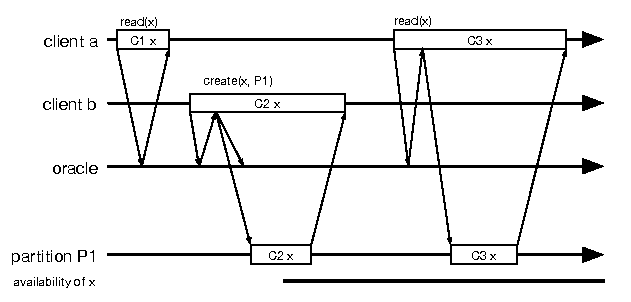
\includegraphics[width=0.6\linewidth]{figures/read_simple}
\end{minipage}
\centering
	\caption{Execution flow of D-SSMR with $create$ command}
\label{fig:read}
\end{figure*}

In the following figures~(\ref{fig:readoverlap}b, \ref{fig:readoverlap}c), where read command $C_1(x)$ comes in the middle of the execution of create command $C_2(x,\ppm_1)$, while the query of $C_1(x)$ comes after multicasts command of $C_2(x,\ppm_1)$. With the knowledge of $x$, Oracle response to the query with a positive answer, therefore there are possibilities that the read command either comes during (eg., fig.~\ref{fig:readoverlap}b) or before (eg., fig.~\ref{fig:readoverlap}c) the execution of actual write command. The SSMR model avoid the problem described in figure~\ref{fig:readoverlap}~(b) by ensuring that the execution of every command is atomic (eg., for every server $s$ in partition $\ppm$ that executes $C$, there is a server $r$ in every $\ppm' \in part(C)$ such that $delivery(C,r) < end(C,s)$. Intuitively, this condition guarantees that the execution of $C_1$ and $C_2$ at $\ppm$ overlap in time). Atomic multicast prevents the problem figure~\ref{fig:readoverlap}~(c) from happening as $deliver(C_2) \prec deliver(C_1)$, that leads to situation described in fig.~\ref{fig:readoverlap}b.

\begin{figure*}
\begin{minipage}[b]{1.0\linewidth} % A minipage that covers the whole width of the page
\centering
      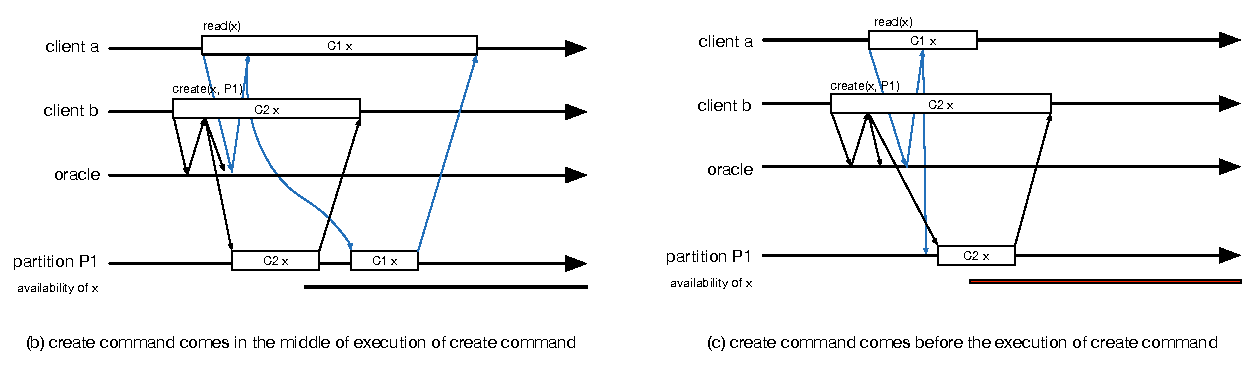
\includegraphics[width=1\linewidth]{figures/read_overlap}
\end{minipage}
\caption{Execution flow of D-SSMR with overlapping read-create commands}
\label{fig:readoverlap}
\end{figure*}


Next figure~(\ref{fig:updateoverlap} a, \ref{fig:updateoverlap} b) depicts the scenario of moving object location from a partition to another. Intuitively, the problem with the execution in fig.~\ref{fig:updateoverlap}a is that read command $C_3(x)$ executes “in between” the execution of $C_2(x,\ppm_2)$ at partitions Px and Py. Before sending $C_3$ to destination partition, client 1 send query to oracle for possible position of $x$, which is $P_1$ at that specific moment, but not correct at the execution time. In D-SSMR, we prevent that from happening by using oracle as the controller for accessing state variable on partitions, by using locking mechanism on oracle for different type of commands. Whenever a client sends a query variable's location $Q(x)$ from oracle for a command $C$, it also requires a lock $L(x)$. Then after the associated process execute command $C$, it also tell Oracle to release the lock $L$, and inform the oracle about the update of $x$ (if there is any).

There are possibilities that a client could fail in the middle of the execution of the command chains, at the moment after requires the lock and before sending the actual $C$ command to partition $P$. In this case, TODO: which one release lock, either oracle or another client that require lock again. 

\begin{figure*}
\begin{minipage}[b]{1.0\linewidth} % A minipage that covers the whole width of the page
\centering
      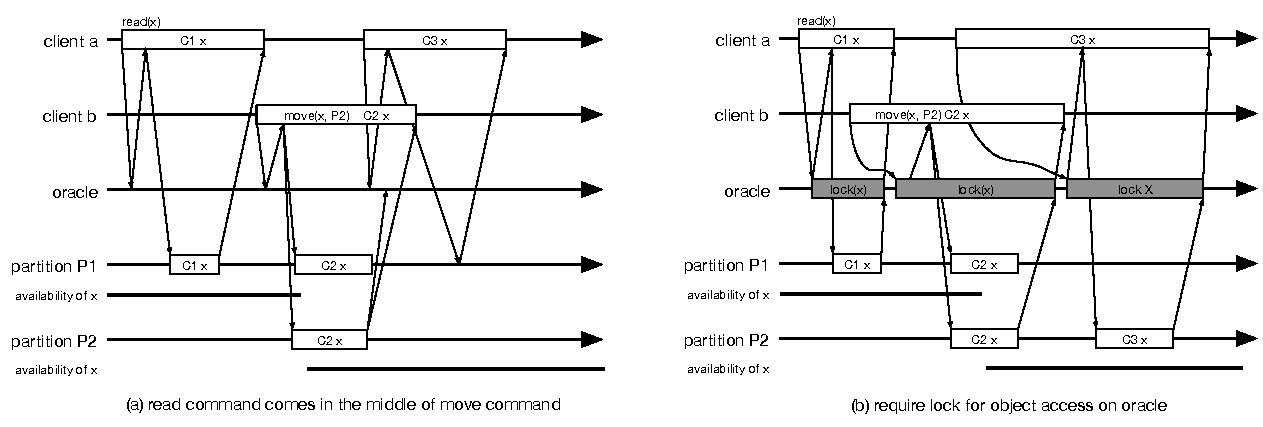
\includegraphics[width=1\linewidth]{figures/update_overlap}
\end{minipage}
\caption{Execution flow of D-SSMR with overlapping read-update commands}
\label{fig:updateoverlap}
\end{figure*}


\subsection{Detailed algorithm}
\label{sec:detailalg}

In Algorithm \ref{alg:dssmr}, we show the basic operation of D-SSMR. 
To submit a command $C$, the client queries an oracle to get set $dests$~(line \ref{algline:query_oracle}, \ref{algline:oracle_response}), which is a superset of $part(C)$ used by the client as destination set for $C$~(line \ref{algline:cli_mcast}). If the $dests$ is empty, client stop the command there. (line \ref{algline:cli_terminate})

Upon delivering $Q(C)$, oracle $O$ runs function $getPart(C)$ which returns a set $\vvm$ of involved state variables of command $C$. If there exists a variable $v_i \in \vvm$ in oracle memory, which indicates the variable $v_i$ exists on a partition $p_i \in \ppm$, oracle reply to client with $p_i$ value, or an empty result otherwise. In addition, upon delivering $C(v, \ppm)$, oracle update its memory with new location of $v$: $\vvm\_part\{v.id\} \leftarrow \ppm$

Upon delivering $C$, server $P$ execute $C$ and reply to the client. 
% Upon delivering $C$, server $s$ in partition \pp\ multicasts $signal(C)$ to $others$, which is the set containing all other partitions involved in $C$ (lines \ref{algline:others} and \ref{algline:mcastsignals}). 
% %The purpose of $signal(C)$ is to let servers in other partitions know that there is a server in \pp\ that started executing $C$. 
% It might happen that $s$ receives signals concerning $C$ from other partitions even before $s$ started executing $C$. For this reason, $s$ must buffer signals and check if there are signals buffered already when starting the execution of $C$. For the sake of simplicity, Algorithm \ref{alg:ssmr} simply initializes such buffers as $\emptyset$ for all possible commands. In practice, buffers for $C$ are created when the first message concerning $C$ is delivered.

% After multicasting signals, server $s$ proceeds to the execution of $C$, which is a sequence of operations that might read or write variables in \vv. The main concern is with operations that read variables, as they may determine the outcome of the command execution. All other operations can be executed locally at $s$. If the operation reads variable $v$ and $v$ belongs to \pp, $s$'s partition, then $s$ multicasts the value of $v$ to the other partitions that delivered $C$ (line \ref{algline:multicastv}). The command identifier $C.id$ is sent along with $v$ to make sure that the other partitions will use the appropriate value of $v$ during $C$'s execution. If $v$ belongs to some other partition $\ppm'$, $s$ waits until an up-to-date value of $v$ has been delivered (line \ref{algline:waitvariable}). Every other operation is executed with no interaction with other partitions (line \ref{algline:executeopck}).

% After executing all operations of $C$, $s$ waits until a signal from every other partition has been received (line \ref{algline:waitsignals}) and, only then, sends the reply back to the client (line \ref{algline:sendreply}). This ensures that $C$ will be execution atomic.



% Upon delivering $C$, server $s$ in partition \pp\ multicasts $signal(C)$ to $others$, which is the set containing all other partitions involved in $C$ (lines \ref{algline:others} and \ref{algline:mcastsignals}). 
% %The purpose of $signal(C)$ is to let servers in other partitions know that there is a server in \pp\ that started executing $C$. 
% It might happen that $s$ receives signals concerning $C$ from other partitions even before $s$ started executing $C$. For this reason, $s$ must buffer signals and check if there are signals buffered already when starting the execution of $C$. For the sake of simplicity, Algorithm \ref{alg:dssmr} simply initializes such buffers as $\emptyset$ for all possible commands. In practice, buffers for $C$ are created when the first message concerning $C$ is delivered.


\begin{algorithm}
\small
%\footnotesize
\begin{distribalgo}[1]
%\STATE \textbf{Algorithm 1:\\} Scalable State-Machine Replication (S-SMR)
\vspace{1mm}

\INDENT{\emph{Initialization:}}
    \STATE  oracle: $\vvm\_part \leftarrow \emptyset$
    % \STATE $\forall C \in \mathcal{K} : rcvd\_signals(C) \leftarrow \emptyset$
    % \STATE $\forall C \in \mathcal{K} : rcvd\_variables(C) \leftarrow \emptyset$
\ENDINDENT

\vspace{1.5mm}

\INDENT{\emph{Command $C$ is submitted by a client as follows:}}
	\STATE multicast query $Q(oracle, C)$ \label{algline:query_oracle} 
    \STATE $dests \leftarrow O(C)$ \label{algline:oracle_response} 
    \IF {$dests$ is $\emptyset$}
    	\STATE terminate $C$ \label{algline:cli_terminate}
    \ELSE
    	\STATE multicast$(dests, C)$ \label{algline:cli_mcast}
    	\STATE wait for response from one server
    \ENDIF
%    \COMMENT{$oracle(C)$ returns a superset of $part(C)$}
\ENDINDENT

\vspace{1.5mm}

\INDENT{\emph{Command $C$ is executed by a oracle as follows:}}
	\INDENT{\textbf{upon} deliver $Q(C)$}
		\STATE $v \leftarrow get part(C)$
		\IF {$v$ in $\vvm\_part$}
			\STATE send reply to client $\vvm\_part\{v.id\}$
		\ELSE
			\STATE send reply to client $\emptyset$
		\ENDIF
	\ENDINDENT

	\INDENT{\textbf{upon} deliver $C(v, \ppm)$}
		\STATE $\vvm\_part\{v.id\} \leftarrow \ppm$
	\ENDINDENT

\ENDINDENT

\vspace{1.5mm}

\INDENT{\emph{Command $C$ is executed by a server in partition \pp\ as follows:}}
	\INDENT{\textbf{upon} deliver$(C)$}	    
		\STATE execute $op$ \label{algline:executeopck}
		\STATE send reply to client \label{algline:sendreply}
	\ENDINDENT
\ENDINDENT

\vspace{1.5mm}
%\vspace{2mm}

\textbf{Algorithm variables:}

\vspace{1mm}

$\vvm\_part$: the set of partitions of all state variables in the system.

\vspace{1mm}

$Q(oracle, C)$: multicast command to oracle for querying involved partition of command C

\vspace{1mm}

$O(C)$: response of oracle that returns a superset of $part(C)$

\vspace{1mm}

$dests$: set of partitions to which $C$ is multicast

\vspace{1mm}

$C(v, \ppm)$: command that create variable $v$ in partition $\ppm$


In the Algoritm \ref{alg:dssmr_with_lock}, we improve the first one with the locking mechanism, let Oracle control access to state variable on partitions. 

\caption{Dynamic Scalable State-Machine Replication with locking (D-SSMR)}
\label{alg:dssmr_with_lock}
\end{distribalgo}
\end{algorithm}


\begin{algorithm}
\small
\begin{distribalgo}[1]
\vspace{1mm}

\INDENT{\emph{Initialization:}}
    \STATE  oracle: $\vvm\_part \leftarrow \emptyset$
    \STATE  oracle: $\vvm\_lock \leftarrow [false]$
    \STATE  oracle: $Q_q \leftarrow \emptyset$
\ENDINDENT

\vspace{1.5mm}

\INDENT{\emph{Command $C$ is submitted by a client as follows:}}
	\STATE multicast query $Q(oracle, C)$ \label{algline:query_oracle} 
    \STATE $dests \leftarrow O(C)$ \label{algline:oracle_response} 
    \IF {$dests$ is $\emptyset$}
    	\STATE terminate $C$ \label{algline:cli_terminate}
    \ELSE
    	\STATE multicast$(dests, C)$ \label{algline:cli_mcast}
    	\STATE wait for response from one server
    \ENDIF
\ENDINDENT

\vspace{1.5mm}

\INDENT{\emph{Command $C$ is executed by a oracle as follows:}}
	\INDENT{\textbf{upon} deliver $Q(C)$} \label{algline:oracle_deliver_C} 
		\STATE $v \leftarrow get part(C)$
		\IF {$\vvm\_lock\{v.id\}$ is false}
			\IF {}
				\STATE require lock  $\vvm\_part\{v.id\} \leftarrow true$
				\STATE send reply to client $\vvm\_part\{v.id\}$
			\ELSE
				\STATE queue $\vvm\_part\{v.id\}$
			\ENDIF
		\ELSE
			\STATE queue command for later execution $Q_q \leftarrow Q(C)$
		\ENDIF
	\ENDINDENT

	\INDENT{\textbf{upon} deliver $C(v, \ppm)$}
		\STATE $\vvm\_part\{v.id\} \leftarrow \ppm$
	\ENDINDENT

	\INDENT{\textbf{upon} deliver $R(v)$}
		\STATE release lock $\vvm\_lock\{v.id\}$
		\IF {$Q_q is not \emptyset$}
			\STATE return to line \ref{algline:oracle_deliver_C} 
		\ENDIF
	\ENDINDENT
\ENDINDENT

\INDENT{\emph{Command $C$ is executed by a server in partition \pp\ as follows:}}
	\INDENT{\textbf{upon} deliver$(C)$}	    
		\STATE execute $op$ \label{algline:executeopck}
		\STATE send reply to client \label{algline:sendreply}
		\STATE send release lock to oracle \label{algline:send_release_lock}
	\ENDINDENT
\ENDINDENT


\vspace{1.5mm}
%\vspace{2mm}

\textbf{Algorithm variables:}

\vspace{1mm}

$\vvm\_part$: the set of locations of all state variables in the system.

\vspace{1mm}

$\vvm\_lock$: the set of lock to variable 

\vspace{1mm}

$Q_q$: queue of query command on oracle

\vspace{1mm}

$Q(oracle, C)$: multicast command to oracle for querying involved partition of command C

\vspace{1mm}

$O(C)$: response of oracle that returns a superset of $part(C)$

\vspace{1mm}

$R(v)$: command send to Oracle to release lock to variable $v$

\vspace{1mm}

$dests$: set of partitions to which $C$ is multicast

\vspace{1mm}

$C(v, \ppm)$: command that create variable $v$ in partition $\ppm$

\caption{Dynamic Scalable State-Machine Replication with locking mechanism}
\label{alg:dssmr}
\end{distribalgo}
\end{algorithm}

\subsection{Performance optimizations}
\label{sec:optm}
TODO: add content, talk about caching

Algorithm 1 can be optimized in many ways. In this section, we briefly mention some of these optimizations and then detail caching.

\begin{figure*}
\begin{minipage}[b]{1\linewidth} % A minipage that covers the whole width of the page
\centering
      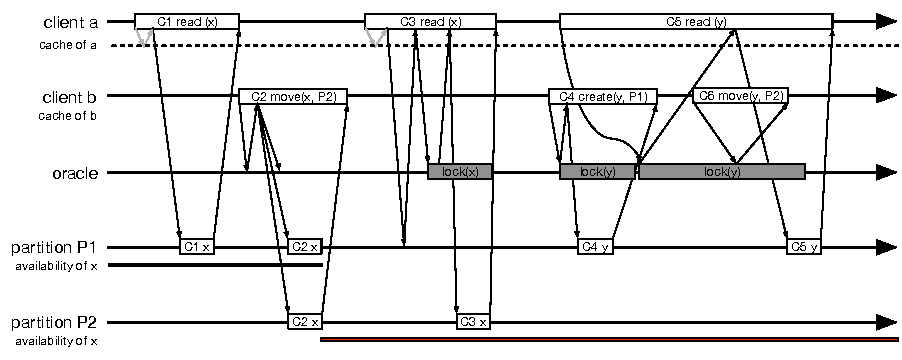
\includegraphics[width=0.85\linewidth]{figures/cache}
\end{minipage}
\caption{Execution flow of D-SSMR with oracle caching on client}
\label{fig:cache}
\end{figure*}

\subsection{Correctness}
\label{sec:correctness}
TODO: add content

\newpage

% why did you have this vvv ?
%\bibliographystyle{splncs03}
\bibliographystyle{ieeetr}
\bibliography{references}
\newpage


\end{document}